\section{Flowchart}
A flowchart is a type of diagram that represents an algorithm, work flow or process, showing the steps as boxes of various kinds, and their order by connecting them with arrows
and the flowchart \ref{fig:openscad-compile} of OpensCAD showing the flow of control and Data in the software and \ref{fig:finalflow} shows the final expected flow chart.

\begin{figure}[H]
\centering
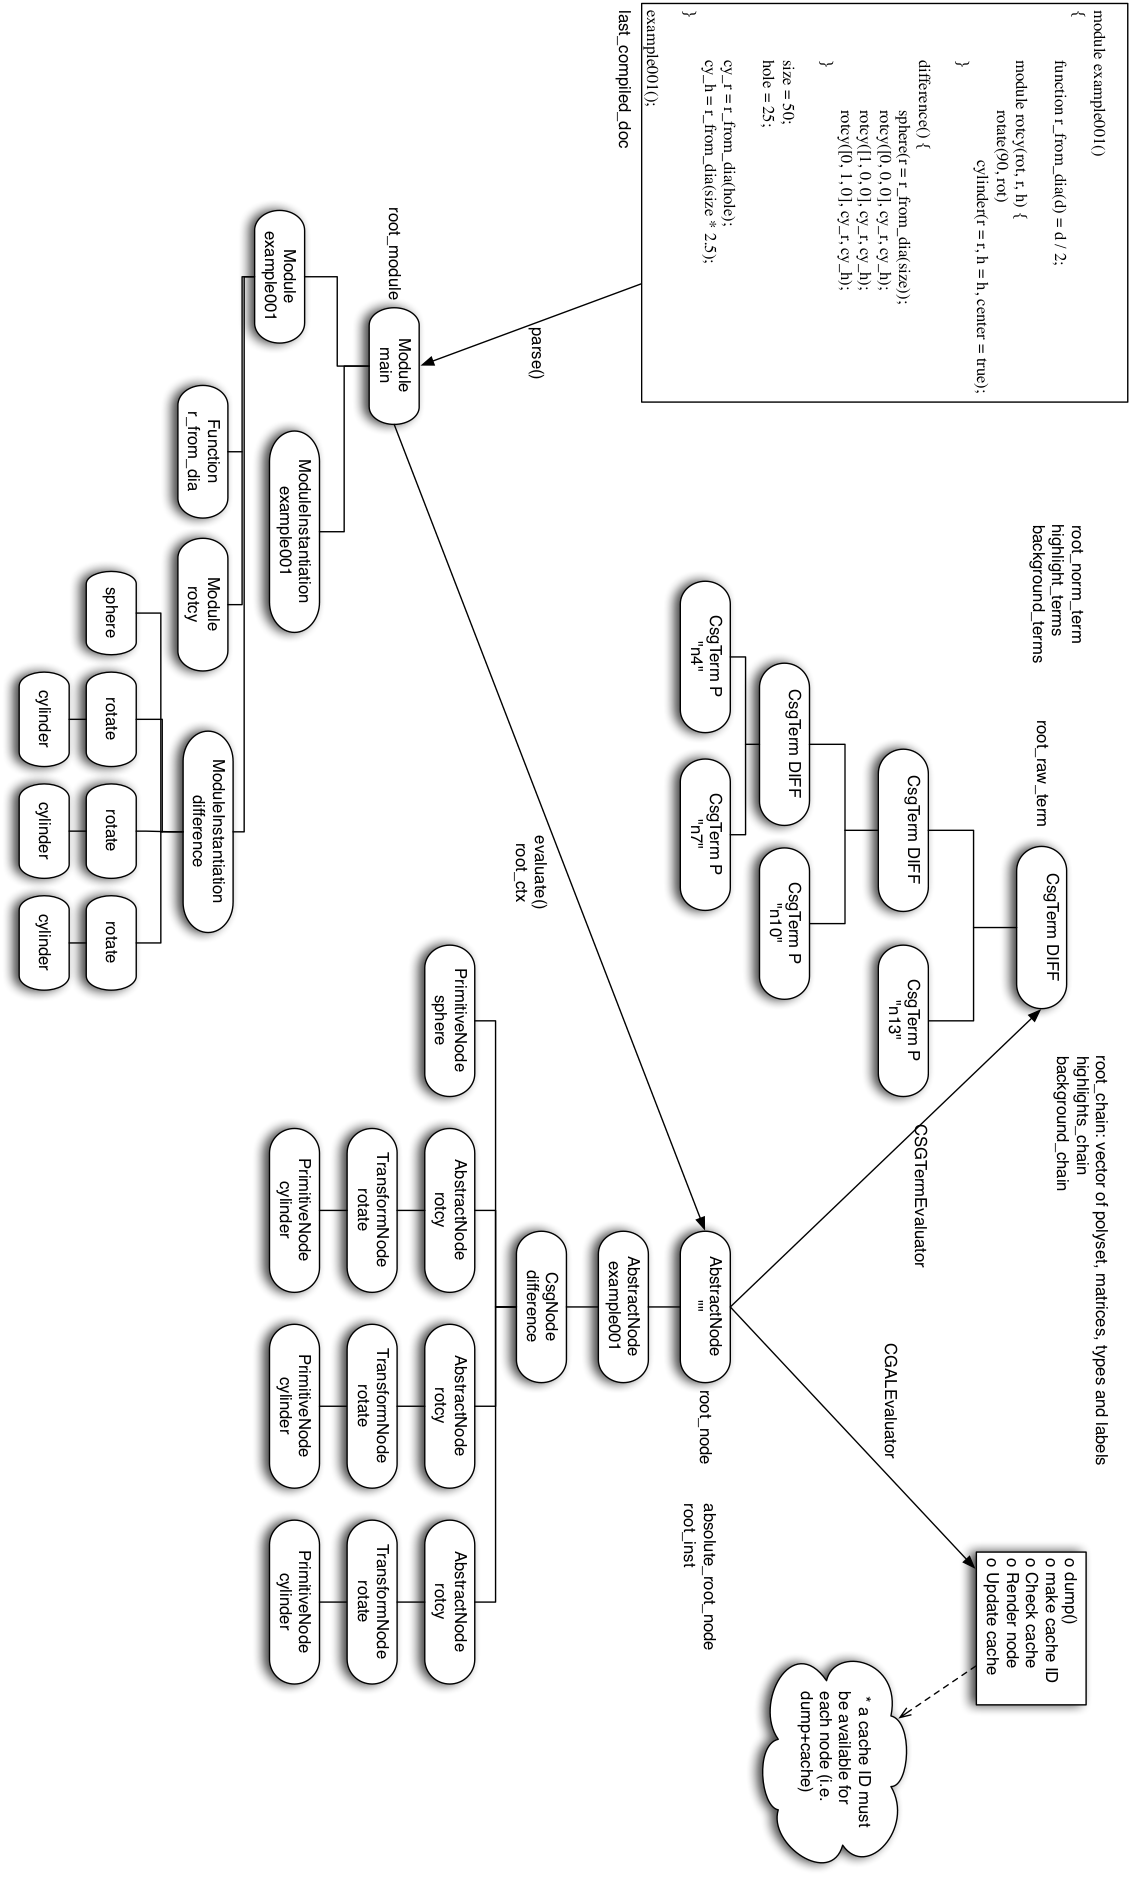
\includegraphics[height=1.37\columnwidth]{images/OpenSCAD-compile.png}
\caption{Detailed flowchart of OpenSCAD}
\label{fig:openscad-compile}
\end{figure}

\begin{figure}[H]
\centering
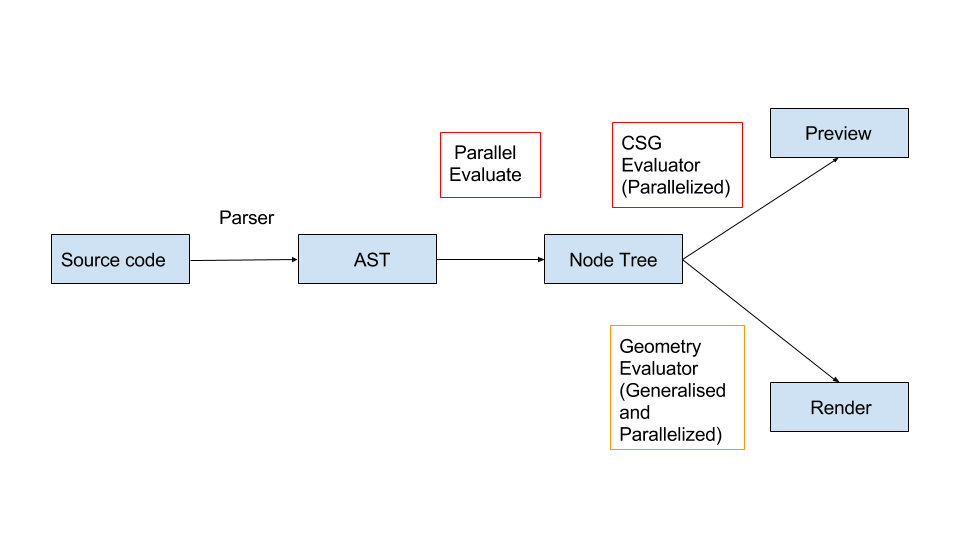
\includegraphics[width=1\linewidth]{images/finalflow}
\caption{Simplefied Final flowchat of OpenSCAD}
\label{fig:finalflow}
\end{figure}

